\chapter{Vector Bundles}

\begin{definition}[Fiber Bundle]
A \textbf{Fiber Bundle} is a topological space $E$, a manifold $M$, and a function $\pi : E \rightarrow M$, where the \textbf{Fiber} $F$ for a point $p \in M$ is $\pi^{-1} (p)$. In order for the set to be a Fiber Bundle, any neighborhood $U$ of $p\in M$, $\pi^{-1}(U)$ is homomorphic to $U \times F$.
\end{definition}

\begin{example} \label{ex:r2} For example $E = \mathcal{R}^2$, $M=\mathcal{R}$, and $\pi: (x,y) \rightarrow x$. See Fig~\ref{fig:r2}
\end{example}

\begin{example} The Mobius strip is a non-trivial bundle where the $M=\mathcal{S}$ and the fiber is $\mathcal{R}$.  See Fig~\ref{fig:mobius}
\end{example}

\begin{figure}
  \begin{subfigure}{.4\textwidth}
  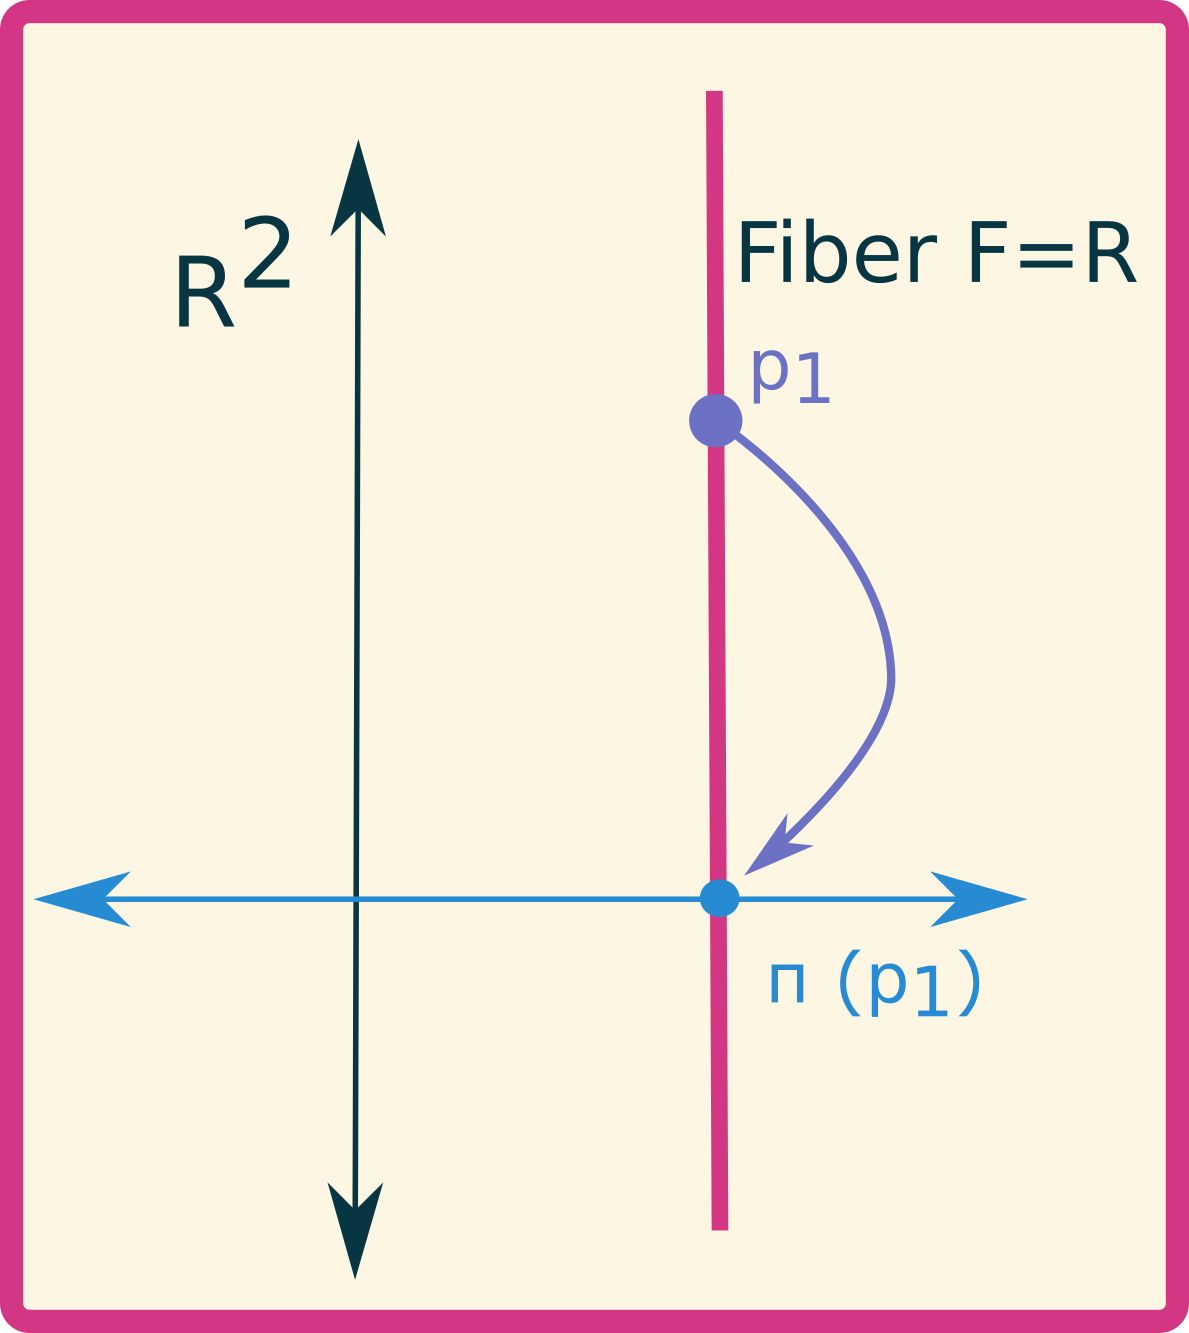
\includegraphics[width=\textwidth]{pics/r2.png}
  \caption{}
  \label{fig:r2}
\end{subfigure}
\begin{subfigure}{.6\textwidth}
  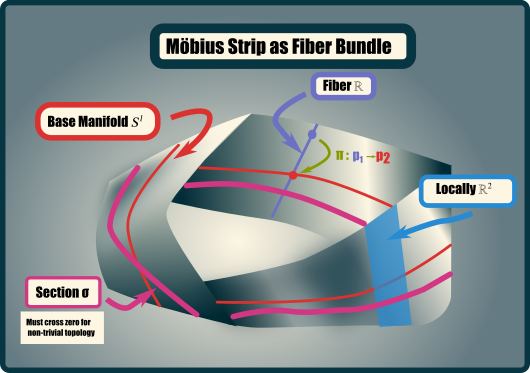
\includegraphics[width=\textwidth]{pics/mobius.png}
  \caption{}
  \label{fig:mobius}
\end{subfigure}
  \label{fig:fiberbundles}
  \caption{a) A simple fiber bundle. b) A Mobius strip is a simple non-trivial fiber bundle.}
\end{figure}

\begin{definition}[Section]
A \textbf{Section} is a function $\sigma : M \rightarrow E$ such that $\pi \cdot \sigma : M \rightarrow M$ is the identity map on $M$.
\end{definition}

\begin{example} Given our vector bundle from Example~\ref{ex:r2},  take the section $\sigma(x) = (x,x^2)$.  If we then apply the $\pi$ projection function, $\pi (x,x^2) = x$.  So our composition would be the identity and $\sigma$ is a valid section.
\end{example}
